\documentclass{standalone}
\usepackage{tikz}
\usepackage{tikz-qtree}
\usepackage[makeroom]{cancel}
\usetikzlibrary{fit}
\usepackage{booktabs}

% ОПИСАНИЕ: модификация старого алгоритма tree overlap чтобы покрывать все деревья 
\begin{document} 
	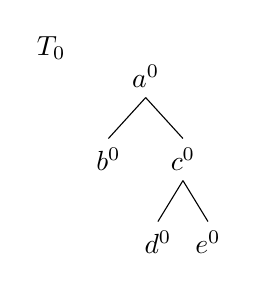
\begin{tikzpicture}

	    
	    \node (x) at (-1.2,0.5) {$T_0$} ;
	    \Tree [.$a^0$
	            [.$b^0$ ] 
	            [.$c^0$
	                [.$d^0$ ] 
	                [.$e^0$ ]
	            ]
	          ]
	\end{tikzpicture}
\end{document} 